%----------------------------------------------------------------------------------------
%	PACKAGES AND OTHER DOCUMENT CONFIGURATIONS
%----------------------------------------------------------------------------------------

\documentclass[a4paper,11pt,twoside,fleqn]{article}

%\usepackage{fourier} % Use the Adobe Utopia font for the document - comment this line to return to the LaTeX default
\usepackage[english]{babel} % For swedish
%\usepackage{amsmath,amsfonts,amsthm} % Math packages

\usepackage[utf8]{inputenc} % Required for swedish characters
\usepackage[T1]{fontenc}
\usepackage{verbatim}
\usepackage{graphicx}
\graphicspath{{./Graphics/}} % Latex looks for graphics here when including

\usepackage{float}
%\usepackage{fullpage}

\usepackage{booktabs}
\usepackage{tabulary}

%\usepackage{siunitx} % For better units and numbers, best use: \SI{41}{\meter\per\second}

%\usepackage{indentfirst}

\usepackage{gensymb}

\usepackage{sectsty} % Allows customizing section commands
\allsectionsfont{\normalfont} % Make all sections centered, the default font and small caps

\usepackage{amsmath} % Allows for equation indentation
\setlength{\mathindent}{1cm}
\setlength{\parindent}{0pt}

\usepackage{geometry}
\geometry{ % Reference(page 3): ftp://ftp.tex.ac.uk/tex-archive/macros/latex/contrib/geometry/geometry.pdf
  top=3cm,				% Top of page to document body
  inner=3cm,
  outer=3cm,
  bottom=3cm,			% Bottom of page to document body
  headheight=3ex,		% Hard to understand, this value seems sufficient
  headsep=2ex,			% Same
}

%\geometry{showframe=true}	% uncomment this line to see document outlines

% Like cleardoublepage, but reverse logic.
\newcommand*\cleartoleftpage{%
  \clearpage
  \ifodd\value{page}\hbox{}\newpage\fi
}

%%%%%%%%%%%%% NICE HEADERS
\usepackage{fancyhdr} % Fancy header and footer
\fancypagestyle{plain}{
\fancyhead{}
\fancyfoot{}
\fancyhead[RO]{\nouppercase{\rightmark}}
\fancyhead[LE]{\nouppercase{\leftmark}}
\fancyfoot[LE,RO]{\thepage}
\renewcommand{\headrulewidth}{0.4pt}
\renewcommand{\footrulewidth}{0.4pt}
}
\pagestyle{plain}


%\numberwithin{equation}{section} % Number equations within sections (i.e. 1.1, 1.2, 2.1, 2.2 instead of 1, 2, 3, 4)
%\numberwithin{figure}{section} % Number figures within sections (i.e. 1.1, 1.2, 2.1, 2.2 instead of 1, 2, 3, 4)
%\numberwithin{table}{section} % Number tables within sections (i.e. 1.1, 1.2, 2.1, 2.2 instead of 1, 2, 3, 4)

%\setlength\parindent{0pt} % Removes all indentation from paragraphs - comment this line for an assignment with lots of text

%----------------------------------------------------------------------------------------
%	TITLE SECTION
%----------------------------------------------------------------------------------------

%\newcommand{\horrule}[1]{\rule{\linewidth}{#1}} % Create horizontal rule command with 1 argument of height

\title{	
\normalfont \normalsize 
%s\textsc{Chalmers University of Technology} \\ [25pt] % Your university, school and/or department name(s)
\huge EDA092 - Lab 2 Report \\ Group A27 \\ % The assignment title
}

\author{Henrik Hugo \& Simon Fransson \\ (\texttt{hhugo@student.chalmers.se, frsimon@student.chalmers.se})} % Your name

\date{\normalsize\today} % Today's date or a custom date

\begin{document}

\maketitle % Print the title
\clearpage
%----------------------------------------------------------------------------------------
%	PART 1
%----------------------------------------------------------------------------------------

\section{One lock}
Measurements done with one lock and proofing why the solution does not yield any deadlocks.
\subsection{Measurements}
As shown in Figure 1 there is a difference between 2 and 4 threads. The measurements are done over 10 executions and taking the average of the execution time. The results shows that it takes more time for the program to finish with more threads. These results are intriguing as one would think that an increased amount of threads would yield in less execution time. This is reasonable because more work should be done in less time. This is however not the case and the reason is because of collisions between the different threads as they try to access the critical section at the same time. This leaves threads waiting for the mutual exclusion variable to become available and not doing anything in the meantime. 

This results in an increase in execution time because the program is spending more time waiting than it is actually executing.

\begin{figure}[h]
	\caption{Measurements for one lock}
	\centering
		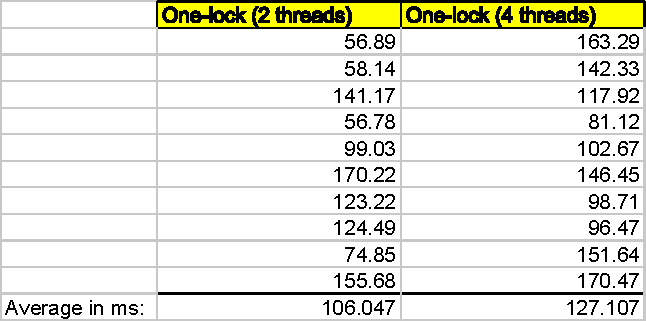
\includegraphics[scale=0.5]{measurements-for-one-lock}
\end{figure}

\subsection{Deadlock}

Question: is deadlock possible to occur? Answer: No.
\\
There are four conditions that needs to be met in order for deadlock to occur:
\begin{itemize}

\item
Mutual exclusion: only one process at a time can use a resource.
\begin{itemize} \item True: Because the \verb+pthread_mutex_lock+ is only allowing one thread at a time to use the queue for enqueuing or dequeuing.
\end{itemize}

\item Hold and wait: a process holding some resource can request additional resources and wait for them if they are held by other processes.
\begin{itemize}
\item False: The enqueue and dequeue functions will not try to request additional resources inside the lock. Also there is only one resource to handle.
\end{itemize}

\item No preemption: a resource can only be release by the process holding it. After that process has completed its task.
\begin{itemize}
\item True: The \verb+pthread_mutex_unlock+ is used for this.
\end{itemize} 

\item Circular wait: there exists a circular chain of 2 or more blocked processes, each waiting for a resource held by the next process in the chain.

\begin{itemize}
\item True: But not in all cases. (4 processes, one resource) 
\end{itemize} 
\end{itemize}

\textbf{Conclusion:} Since at least one of the conditions is broken, deadlock can not occur.

\clearpage

%----------------------------------------------------------------------------------------
%	PART 2
%----------------------------------------------------------------------------------------

\section{Two locks}

%------------------------------------------------

\subsection*{Blah}

Compare against one lock:

\subsection*{\textbf{Deadlock}}

Question: is deadlock possible to occur? Answer: No.
\\
The same conclusion as from part 1 can be drawn again. The difference with the two locks does not introduce any complications. This is because the two locks are independent of each other. It might have been a problem if once one lock had been acquired to start and trying to acquire the other lock as well. However since the implementation is not done in this way, the problem does not arises.

%----------------------------------------------------------------------------------------

\end{document}